\documentclass{article}
\usepackage[utf8]{inputenc}
\usepackage{amsmath}
\usepackage{amsthm}
\usepackage[margin=10px]{geometry}
\usepackage{graphicx}
\usepackage{enumitem}
\setlength{\parindent}{0pt}
\setlist{itemsep=0.05em, topsep=0.2em}

\title{Networked Systems}
\author{}
\date{}

\begin{document}

% \footnotesize

\subsection*{The Changing Internet}

% 1b
\textbf{Networked System}: A cooperating set of autonomous computing devices that exchange data to perform some application goal.

\begin{figure}[h]
    \centering
    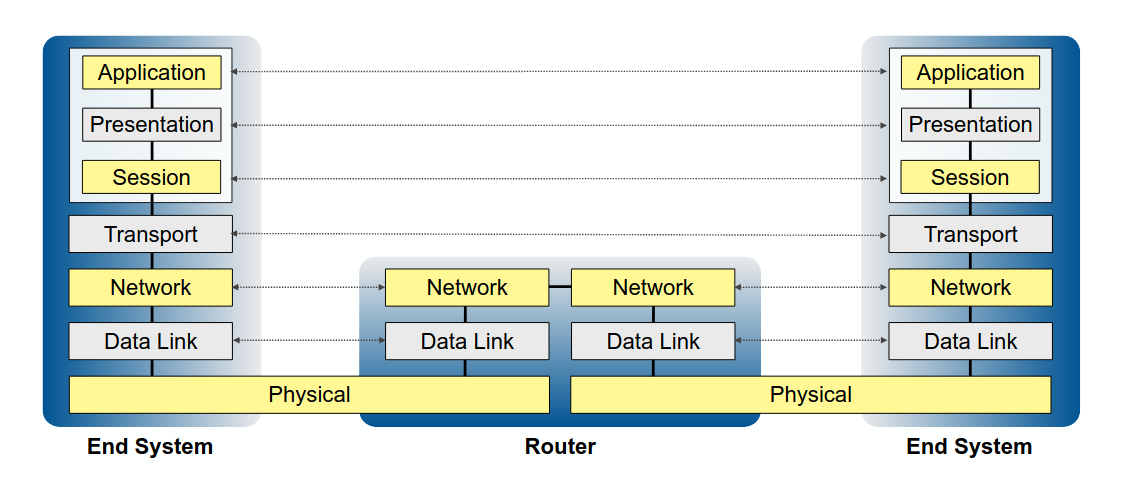
\includegraphics[width=0.35\textwidth]{assets/osi-model.png}
    \caption{OSI Reference Model}\label{fig:osi-model}
\end{figure}

\textbf{OSI Reference Model}

Application Layer, Presentation Layer, Session Layer, Transport Layer, Network Layer, Data Link Layer, Physical Layer.

\textbf{Note}: Real networks don't follow the OSI Reference Model.

\vspace{\baselineskip}
% 1c

\textbf{Physical Layer}:

Raw bits are transmitted over a physical medium.

\textbf{Nyquist's Theorem}: The maximum bitrate of a channel is described by Nyquist's theorem:
\[
R_{\max} \leq 2B \log_2 V
\]
$B$ = bandwidth of the channel,
$V$ = number of discrete values per symbol

Maximum data rate only reached with a noise-free channel

\textbf{Baseband Data Encoding}
\begin{itemize}
    \item \textbf{NRZ}: 0 is represented by no change in voltage, 1 is represented by a change in voltage. Easy to miscount long runs of same value.
    \item \textbf{Manchester}: Encoding: 0 is represented by a transition from high to low, 1 is represented by a transition from low to high.
    \item \textbf{Modulation}: Allows multiple signals on a channel, modulated onto carriers of different frequency.
\end{itemize}

\textbf{Modulation} is the process of encoding data onto a carrier wave. You can use \textbf{amplitude}, \textbf{frequency}, or \textbf{phase} to encode data.

\textbf{Data Link Layer}
Provides framing, addressing, media access control, error detection, and flow control.
\textbf{Framing}: Separate the bitstream into meaningful frames of data.

\begin{figure}[h]
    \centering
    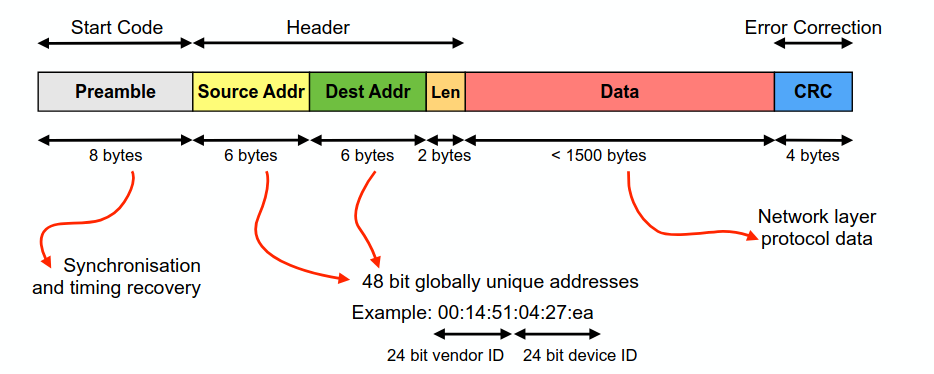
\includegraphics[width=0.4\textwidth]{assets/ethernet-frame.png}
    \caption{Ethernet Frame}\label{fig:ethernet-frame}
\end{figure}

\textbf{Media Access Control}: How devices share the channel. If another transmission is active, the device must wait until the channel is free.
If the link is idle, send data immediately.

% 1d
\textbf{Network Layer}

Provides routing, addressing, and packet switching. Internet Protocol (IP).

\textbf{IPv4}: 32-bit address space. Fragmentation difficult at high data rates.

\textbf{IPv6}: 128-bit address space. No in-network fragmentation. Simple header format, larger header size.

\textbf{Routing}: Each network administered separately {-} an autonomous system (AS), different technologies and policies.

% 1e
\textbf{Transport Layer}

Provides end-to-end error recovery, flow control, and multiplexing.

\textbf{TCP}: Connection-oriented, reliable, in-order delivery, flow control, congestion control.

\textbf{UDP}: Connectionless, unreliable, out-of-order delivery, no flow control, no congestion control.

% 1f
\textbf{Session Layer}

Provides session establishment, maintenance, and termination.

\textbf{Managing Connections}: How to find participants in a connection, how to setup and manage the connection.


\textbf{Presentation Layer}

Managing the presentation, representation, and conversion of data.


\textbf{Application Layer}

Provides the interface to the application. Deliver email, stream video, etc.
\textbf{Happy Eyeballs}: The process of trying multiple connections to a server to find one that is available.


\clearpage

\subsection*{Connection Establishment in a Fragmented Network}

% 2a
\textbf{TCP}

Transport layer protocol, provides a \textbf{reliable} ordered byte stream service over the \textbf{best-effort IP network}.
Provides congestion control to adapt to network capacity.

TCP segments carried as data in IP packets.
IP packets carried as data in link layer frames.
Link layer frames delivered over physical layer.

\begin{figure}[h]
    \centering
    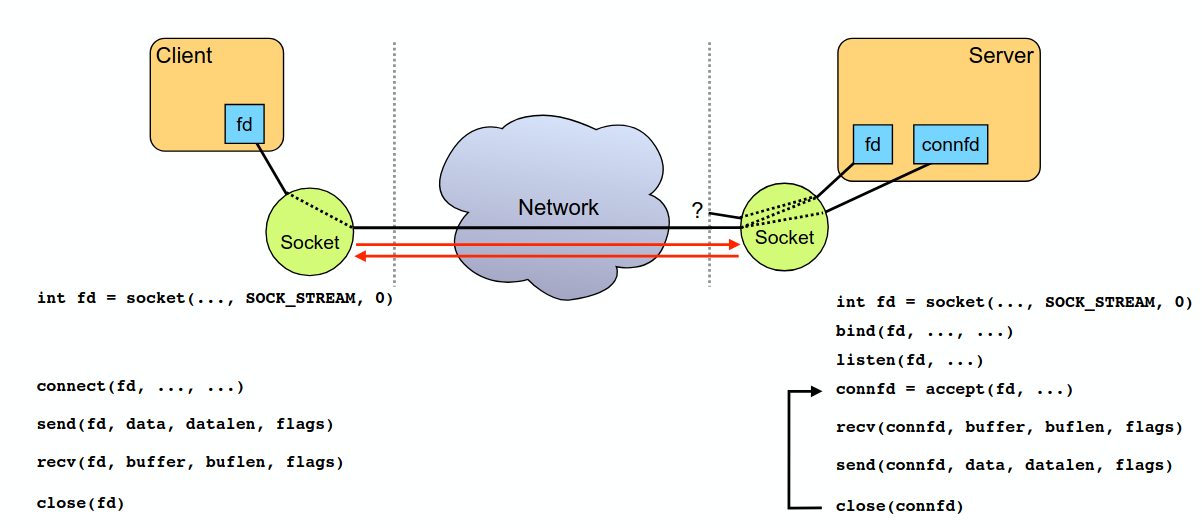
\includegraphics[width=0.4\textwidth]{assets/tcp-programming-model.png}
    \caption{TCP Programming Model}\label{fig:tcp-programming-model}
\end{figure}

Lost packets are retransmitted, \textbf{ordering is preserved}, \textbf{message boundaries are not preserved}.

As RTT increases, benefits of increasing bandwidth reduce.
For example, with a 300ms RTT, increasing bandwidth from 15Mbps to 1Gbps results in only a 22\% reduction in page download time.

\textbf{TCP Connection Establishment}

In the SYN, the client sends a random sequence number.
In the SYN-ACK, the server sends a random sequence number.
In the ACK, the client sends the sequence number of the next byte it expects to receive.
Used to synchronise the sequence numbers.
For short connections, the overhead of the handshake is significant.

\vspace{\baselineskip}
% 2b
\textbf{Impact of TLS on Connection Establishment}

HTTP sends and retrives data immediatly once the TCP connection is open.
HTTPS opens a TCP connection, then negotiates secure parameters using TLS.\@

TLS v1.3: extra 1RTT, TLS v1.2: 2RTT.\@

\vspace{\baselineskip}
% 2c
\textbf{Peer-to-peer Connections}

You should be able to run a TCP server on any device, and TCP, UDP based peer-to-peer applications.
Peer-to-peer connetion establishment is \textbf{difficult} due to network address translation (NAT).

\textbf{NAT} is a work around for the shortage of IPv4 addresses, it allows several devices to share a single public IP address.
ISP assigns new range of IP addressses to customer.
The way sub-network addressing was supposed to work, is that we would have enough IP addresses so that we could have
unique global IP addresses for each device.

Records the mapping, so the reverse changes can be made to any incoming replies as they traverse the NAT in the reverse direction.

\vspace{\baselineskip}
% 2d
\textbf{Problems due to Network Address Translation}

Client-server applications with client behind NAT work without changes {-} web and email.

Client-server applications with server behind NAT fail {-} need explicit port forwarding.

Hard-coding IP addresses, rather than DNS names, in configuration files and application is a bad idea.

Outgoing connections \textbf{create state in NAT}, so replies can be translated to reach the correct host on the private network.
No state for incoming connections. NAT cant't know where to forward incoming connections, without manual confiuration.
UDP not connection-oriented; NAT can't detect the end of a flow, so use short timeout to cleanup state once UDP flow has stopped

\vspace{\baselineskip}
% 2e
\textbf{NAT Traversal and Peer-to-Peer Connections Establishment}

NATs support outbound connections from client to server.

Incoming connections fail, since NAT cannot know how to translate the incoming packets

Peer-to-peer connections can succeed if both NATs think a client server connection is being opened, and the response is coming from the server

Peers connect to referral server on public network, use server to discover the NAT bindings: \textbf{binding discovery}.

\textbf{Exchange candidate} addresses with peer via the referral server: address discovery.

Peers systematically \textbf{probe connectivity}, try to estrablish a connection using every possible combination of candidate addresses.

\textbf{NAT binding discovery}: Requesting a server to tell you the public IP address and port number that you're on.

\textbf{Candidate Exchange}: Each host discovers its candiate IP addresses/port. Peers exchange candidate addresses.

They make TCP connections to the relay server and exchange data over those connections, to reduce latency and to preserve privacy.

\textbf{The ICE algorithm}: try $connect()$ with each candidate address, until a connection is established.
Connection requests sent from a host that passes through a NAT will open a binding that allows a response, even if the connection fails.

\clearpage

\subsection*{Secure Communications}

% 3a
\textbf{The Need for Secure Communications}

Numerous organisations monitor network traffic.
Mechanisms that protect privacy against malicious attackers will also prevent monitoring.
Preventing protocol ossification: network operators deploy middleboxes to monitor or modify traffic.
These middleboxes must inderstand the protocols, this creates ossification.
The more of a protocol that is encrypted, the easier it is to change.

\vspace{\baselineskip}
% 3b
\textbf{Principles of Secure Communication}

How to deliver message from sender to receiver securely:

\begin{itemize}
    \item \textbf{Avoid eavesdropping}: encrypt to provide confidentiality
    \item \textbf{Avoid tampering}: authentiate to ensure the message is not modified in transit
    \item \textbf{Avoid spoofing}: validate identity of sender
\end{itemize}

Use encryption to make data useless if intercepted.

\textbf{Symmetric Cryptography}: Same key used for encryption and decryption. Very fast, suitable for bulk data.

\textbf{Public-Key Cryptography}: Different keys for encryption and decryption. Very slow.

\textbf{Hybrid Cryptography}: combines the strengths of public-key and symmetric encryption:
a small symmetric key is securely shared using slower public-key encryption,
and then that key is used for fast, secure communication using symmetric encryption.
This approach ensures both confidentiality and performance.

\textbf{Digital Signatures}: Sender generates a digital signature,
sender calcualte the cryptographic hash of the message,
sender encrypts the hash with their private key.
message and its digital signature are sent to the receiver using hybrid encryption.
Reciever decrypts the message,
reciever calcualtes the cryptographic hash of the message,
reciever decrypts the digital signature using the senders public key,
if the signature is valid and the message is unchanged, the reciever can be sure that the message was sent by the claimed sender.

\textbf{Public key infrastructure (PKI)} verifies digital signatures.

\vspace{\baselineskip}
% 3c
\textbf{Transport Layer Security (TLS)}

Used to encrypt and authenticate data carried within a TCP connection.
TLS handshake runs within a TCP connection.
TLS doesnt encrypt TCP headers.

\textbf{ClientHello} is sent with the ACK, \textbf{ServerHello} is sent in response, \textbf{Finished} message concludes.

\textbf{ClientHello} signals TLS v1.2 but header indicates TLS v1.3, provides the cryptographic algorithms the client supports, provides the name of the server to which the client is connecting, no data.

\textbf{ServerHello} provides the cryptographic algorithm the server supports, from the ones the client supports, provides the servers public key and digital signature.

\textbf{Finished} provides clients public key, may contain data sent from client to server.

\textbf{TLS record protocol}: splits the data into records ($< 2^{14}$ bytes), encrypts each record with a record layer key. Does not provide record boundaries.

\textbf{0-RTT}: If a client and server have previously communicated, they can re-use a key (0-RTT).

\textbf{Limitations of TLS}: does not encrypt server name, operates within TCP connection, relies on a PKI to validate public keys.


\clearpage

\subsection*{Improving Secure Connection Establishment}

% 4a
\textbf{Limitations of TLS}

TLS still has some limitations:
\begin{itemize}
    \item Connection establishment is still relatively slow, and so first data is sent 2x RTT after the start.
    \item Connection establishment leaks potentially sensitive metadata
    \item The protocol is ossified due to middlebox interference.
\end{itemize}

\textbf{0-RTT Connection Reestablishment}

Reuse a preshared key agreed in previous TLS session.
Server sends a \textbf{PreSharedKey} with a \textbf{SessionTicket} to identify the key.
When reestablishing a connection: Client sends \textbf{SessionTicket}, data encrypted using corresponding
\textbf{PreSharedKey}, along with \textbf{ClientHello}. The server uses \textbf{SessionTicket} to find saved \textbf{PreSharedKey},
decrypt the data.
0-RTT data sent with \textbf{ClientHello} using a \textbf{PreSharedKey} is not forward secret.
If a session where \textbf{PreSharedKey} is distributed is compromised,
0-RTT data sent using that key in future connections will also be compromised.

\textbf{TLS Metadata Leakage}: server name and \textbf{PreSharedKey} are not encrypted

\textbf{TLS Protocol Ossification}: Some TLS servers fail if \textbf{ClientHello} uses unexpected version number.

TLS 1.3 says its using TLS 1.2, but it says in the header that it is using TLS 1.3.

\textbf{How to Avoid Protocol Ossification}:
\textbf{GREASE}: Generate random extensions and sustain extensibility: send random extensions that are ignored.

\vspace{\baselineskip}
% 4b
\textbf{QUIC Transport Protocol}

What's wrong with TLS v1.3 over TCP\@?
Slow to connect {-} due to sequential TCP and TLS handshakes,
Leaks some metadata,
Ossified and hard to extend.

QUIC aims to replace TLS v1.3 and TCP with a single secure transport protocol.
Reduce latency by overlapping TLS and transport handshake,
Avoid metadata leakage via pervasive encryption,
Avoid ossification via systematic application of GREASE and encryption

QUIC replaces TCP, TLS, and parts of HTTP
QUIC sends and receives streams of data within a connection.

Up to $2^{62}$ different streams in each direction in a single QUIC connection
A connection comprises QUIC packets sent within UDP datagrams.

\textbf{QUIC Headers}. QUIC packets can be long header packets or short header packets.
\textbf{Long header} packets are used to establish a connection.
\textbf{Short header} packets are used for all packets sent after the TLS handshake is complete.
Four different long-header packet types, denoted by the TT field in the header:
Initial {-} initiates connection, starts TLS handshake,
0-RTT {-} idempotent data sent with initial handshake, when resuming a session,
Handshake {-} completes connection establishment,
Retry {-} used to force address validation.
The is one short header packet defined in QUIC\@:
1-RTT {-} Used for all packets sent after the TLS handshake is complete. QUIC packet contain an encrypted sequence of frames

\textbf{QUIC Frames}: QUIC packet contain an encrypted sequence of frames.


\vspace{\baselineskip}
% 4c
\textbf{QUIC Connection Establishment}

A QUIC connection proceeds in two phases: handshake and data transfer.

\textbf{C} $\rightarrow$ \textbf{S}: QUIC Initial packet

\textbf{S} $\rightarrow$ \textbf{C}: QUIC Initial and Handshake Packet

\textbf{C} $\rightarrow$ \textbf{S}: QUIC Initial, Handshake, and 1-RTT Packet

Initial packet contains a CRYPTO frame that contains TLS ClientHello or ServerHello, also synchronises the client and server state.

QUIC Initial packets also carry optional Token.
Server can refuse the initial connection attempt, and send a Retry packet containing a Token.
Client must then retry the connection, providing the Token in its Initial packet.

QUIC supports TLS 0-RTT session re-establishment: QUIC Initial packet contains CRYPTO frame with a TLS ClientHello
and a SessionTicket QUIC 0-RTT packet included in the same UDP datagram contains a STREAM frame carrying idempotent 0-RTT data:


\textbf{Data Transfer}. After handshake has finished, QUIC switches to sending short header packets.
The short header contains a Packet Number field, Packet numbers increase by one for each packet sent.

ACK frames indicate received packet numbers. QUIC packet numbers count packets sent; TCP sequence numbers count bytes of data sent.
QUIC never retransmits packets {-} retransmits frames sent in lost packets in new packets, with new packet numbers.
QUIC sends acknowledgements of received packets in ACK frames.
Sent inside a long- or short-header packets; unlike TCP, not part of headers.
Indicate sequence numbers of QUIC packets that were received, not frames
Data is sent within STREAM frames, sent within QUIC packets, contains a stream identifier, offset of the data, data length and data.

\vspace{\baselineskip}
% 4d
\textbf{QUIC over UDP}

Why run QUIC over UDP\@? To ease end-system deployment.
To work around protocol ossification due to middleboxes.
Entire packet except invariant fields and the last 7-bits of the first byte is encrypted.
QUIC authenticates all data.
\textbf{Why is QUIC desirable?}.
Reduces secure connection establishment latency.
Reduces risk of ossification; easy to deploy.
Supports multiple streams within a single connection.
\textbf{Why is QUIC problematic?}.
Libraries and support new, poorly documented, and frequently buggy.
CPU usage is high compared to TLS-over-TCP\@.

\clearpage

\subsection*{Reliability and Data Transfer}

% 5a
\textbf{Packet Loss in the Internet}

The Internet is a best effort packet delivery network {-} \textbf{it is unreliable}.
IP packets may be lost, delayed, reordered, or corrupted in transit.
Only put functionality that is absolutely necessary in the network, leave everything else to end systems.
If a connection is to be reliable, it cannot guarantee timeliness.
If a connection is to be timely, it cannot guarantee reliability.

\vspace{\baselineskip}
% 5b
\textbf{Unreliable Data Using UDP}

The $sendto()$ call sends a single datagram.
Each call to $sendto()$ can send to a different address, even though they use the same socket.
The $recv()$ call may be used to read a single datagram, but doesn't provide the source address of the datagram.
Most code uses $recvfrom()$ instead {-} this fills in the source address of the received datagram.
UDP does not attempt to provide sequencing, reliability, or timing recovery.

The \textbf{protocol built on UDP} is responsible for correcting the order, detecting duplicates and repairing loss.
The protocol running within UDP generally includes a sequence number to support this.

\vspace{\baselineskip}
% 5c
\textbf{Reliable Data Using TCP}

TCP ensures data delivered reliably and in order.
TCP sends acknowledgements for segments as they are received; retransmits lost data.
TCP will recover original transmission order if segments are delayed and arrive out of order.

\textbf{TCP Segments and Sequence Numbers}. Data is split into segments, with a sequence number, each placed in a TCP packet.
TCP packets are sent in IP packets.
Sequence numbers start from the value sent in the TCP handshake.

Calls to $send()$ don't directly map to TCP segments.
If data given to $send()$ is small, TCP might wait to send the data, combining it with later data into a single larger segment.

Segments sent to acknowledge each received segment {-} contains acknowledgment number indicating sequence number of the next
contiguous byte expected.
If a packet is lost, subsequenc packets will generate duplicate acknowledgements.
Can send delayed acknowledgements if there is no data to send in reverse direction.

If data is being sent, but no acknowledgement return, then either reciever or network has failed.
TCP treats \textbf{a timeout} as an indication of packet loss and retransmits unacknowledged segments.
\textbf{Loss Detection}: TCP treats a triple duplicate acknowledgement {-} four consecutive acknowledgements for the same sequence
number {-} as an indication of packet loss.

\textbf{Head-of-line Blocking in TCP}: TCP segments are sent in order, if a segment is lost, all subsequent segments are held up.
Significant latency increase.

\vspace{\baselineskip}
% 5d
\textbf{Reliable Data Transfer with QUIC}

QUIC delivers several ordered reliable byte streams within a single connection.
Order is not preserved between streams within a QUIC connection.

Each QUIC packet has a \textbf{packet number}.
Within each space, packet number starts at zero, increases by one for each packet sent.
QUIC doesn't preserve message boundaries in streams.
If data written to stream is too big for a packet, it will be split across multiple packets.
If data written to stream is too small for a packet, it may be delayed and sent with other data to fill complete packet.
Acknowledgements can be delayed.
Acknowledgements contain ranges.
Like TCP Selective Acknowledgement extension.

QUIC does \textbf{not retransmit lost packets}. Every packet has a unique packet numner and is only transmitted once.
Packets are declared lost when at least three later packets have been acknowledged.
QUIC transmits lost data in new packets with \textbf{new packet numbers}.

\textbf{Head-of-line Blocking in QUIC}: QUIC segments are sent in order, if a segment is lost, all subsequent segments are held up.
Significant latency increase.

\clearpage

\subsection*{Lowering Latency}

% 6a
\textbf{TCP Congestion Control}

\textbf{Principles}: packet loss as a congestion signal, additive increase, multiplicative decrease.

\textbf{IP Routers} perform \textbf{Routing} (receive packets and determine route to destination) and
\textbf{Forwarding} (enqueue packet on outgoing link).
\textbf{Queues shrink} if packets are forwarded faster then they arrive.
\textbf{Queueing delay} is packets arrrive faster than they can be forwarded.
\textbf{Packets are discarded if the queue is full}.
Congestion control uses packet loss as a congestion signal.

\textbf{ACK clocking}: each acknowledgement `clocks out' the next packet. TCP uses window-based congestion control.

\textbf{AIMD Algorithm}: Additive Increase, Multiplicative Decrease.

TCP uses window-based congestion control.
Maintains a \textbf{sliding window} onto the available data that determines how much can be sent according to the AIMD algorithm.
Ideally the sliding window is $bandwidth \times delay$.
Each returning acknowledgement for new data slides the window along, releasing next packet for transmission → if window sized
correctly, each acknowledgement arrives just in time to release next packet.
Slow start then congestion avoidance.
Gives approximate equal share of the bandwidth to each flow sharing a link.

\vspace{\baselineskip}
% 6b
\textbf{TCP Reno}

\textbf{Congestion window}: number of packets to be sent before an acknowledgement arrives.
\textbf{Initial window} is typically 1{-}10 packets.
Use \textbf{slow start} by doubling the congestion window after each acknowledgement until a packet is lost,
then reset sending rate to last know good rate.

Then switch to \textbf{congestion avoidance}: linear increase (+1) in window size until a packet is lost, then multiplicative decrease (*0.5)
If a packet is lost and detected via timeout: reset to initial window size.
$timeout = \max(1 second, average RTT + (4 x RTT variance))$
Effective at keeping bottleneck link fully utilised.
Trades some extra delay to maintain throughput.
Congestion avoidance phase takes long time to use increased capacity.
Performs poorly on fast long-distance networks.

\vspace{\baselineskip}
% 6c
\textbf{TCP Cubic}

More aggresive (multiplicative decrease 0.7).
$W_{\text{cubic}} = C {(t - K)}^3 + W_{\text{max}}$.
$W_{\text{max}}$ window size before packet loss.
$t$ time since packet loss.
$K$ time to increase window back to $W_{\text{max}}$.
$C = 0.4$ constant to control fairness to Reno.

\vspace{\baselineskip}
% 6d
\textbf{TCP Vegas}

\textbf{Delay-based Congestion Control}.
Watches for the increase in delay as the queue starts to fill up and slows down before the queue overflows.
Still uses slow start.
Measure BaseRTT, Calculate ExpectedRate = w / BaseRTT, measure ActualRate.
If ExpectedRate {-} ActualRate < R1 then additive increase to window.
If ExpectedRate {-} ActualRate > R2 then additive decrease to window.
Since Reno and Cubic are aggressive, this forces Vegas to slow down and the cycle repeats until rate drops to zero.
So Vegas is not used. TCP Bottleneck Bandwidth \& RTT attempts to make delay-based congestion work.

\vspace{\baselineskip}
% 6e
\textbf{Explicit Congestion Notification (ECN)}

Why not have the network tell TCP congestion is occurring? ECN field in IP header.
00 doesnt support.
01 ECN capable.
11 congestion occurs.
Routers signal congestion before queues overflow.

\vspace{\baselineskip}
% 6f
\textbf{Impact of propagation delay on latency}

Time packets spend in queues.
Time packets spend propagating down links between routers.

\clearpage

\subsection*{Real-time and Interactive Applications}

% 7a
\textbf{Real-time Media Over The Internet}.

Real-time Traffic must be delivered by a certain time, must be \textbf{loss tolerant}.
It requires \textbf{predicable timing}.

For \textbf{streaming applications}, the content may take a few seconds to load but should be smooth once it starts.
Trade-off between frame rate and frame quality.

\textbf{Interactive converencing} has tight latency bounds.
One-way mouth-to-ear delay \textbf{$\sim$150ms} maximum for telephony.
Video converencing want to lip-sync audio and video.
Audio should be no more than \textbf{15ms} ahead or \textbf{45ms} behind.
Speech coding data rate can be 10s of kbps, but should be \textbf{$\sim$100ms}.
Video frame rate can be between \textbf{25} and \textbf{60fps}.

Many transfers are \textbf{elastic} {-} faster is better, but it doesn't matter what rate the congestion control selects.
Real-time traffic is \textbf{inelastic}, has a minimum and maximum rate.

Reserving network capacity makes using the network more expensive.

\vspace{\baselineskip}
% 7b
\textbf{Interactive Applications}

\textbf{Speech data} is highly loss tolerant, loss concealment can hide 10\%--20\% packets loss.
\textbf{Video} packet loss is hard to conceal.

\textbf{Media Transmission Path}
Frames of media data are captured periodically.
Codec compresses media frames.
Compressed frames fragmented into packets.
Transmitted using RTP inside UDP packets.
RTP protocol adds timing and sequencing, source identification, payload identification.
Transmitted over the network.

UDP packets containing RTP protocol data arrive separated according to sender.
Channel coder repairs loss using forward error correction.
Playout buffer used to reconstruct order, smooth timing.
Media is decompressed, packet loss concealed, and clock skew corrected.
Recovered media is rendered to user.
\textbf{Real-time Transport Protocol (RTP)}
Usual TLS handshake but within UDP packets.
Payload formats.
Each packet should be independently usable

\vspace{\baselineskip}
% 7c
\textbf{WebRTC}

Data Channel provides a peer-to-peer data channel.
A signalling protocol is needed to find the peer and establish the paths.
The control protocol needs to describe the communication session expected.
\textbf{Session description protocol (SDP)} provides a standard format for such data.
SDP Offer: Description of the communication session expected by the offerer.
SDP Answer: subsets of the offer, and confirms willingness to communicate.
SDP was not designed to express options and alternatives.
\textbf{Session Initiation Protocol (SIP)} is used to find the peer and establish the paths.
SIP is used to describe the communication session expected.
SIP was designed to express options and alternatives.
\textbf{WebRTC} is an alternative signalling protocol.

\vspace{\baselineskip}
% 7d
\textbf{Streaming Video}

RTP and RTSP offer low latency, but HTTPS is used for easier CDN support despite higher latency.
\textbf{Content Delivery}:
CDNs are optimized for HTTP, not RTP\@.
\textbf{HTTP Adaptive Streaming (DASH)}:
Video split into \~10s chunks at multiple bitrates. Clients pick bitrate based on network speed.
\textbf{DASH and TCP}:
TCP controls congestion fast (RTT), DASH adapts slowly (~10s). Start with low quality, adjust later.
\textbf{Latency}:
Caused by chunk size, buffering, encoding, and TCP retransmissions.
\textbf{Compression Trade-off}:
Smaller chunks reduce latency but waste space due to frequent large I-frames.
\textbf{Future}:
WebRTC (low latency RTP in browsers) and QUIC (YouTube uses it) are the future for video.

\clearpage

\subsection*{Naming and the Tussle for Control}

\vspace{\baselineskip}
% 8a
\textbf{DNS Name Resolution}

IP packets contain addresses, not names.
\textbf{Domain name system (DNS)} is a distributed database; maps names to IP addresses.
\textbf{DNS name structure}: \texttt{<subdomain>.<top-level domain>.<dns root>}.
The \textbf{root servers} advertise the top-level domains.
Resolvers are pre-configured with the IP addresses of the root servers.
They have well-known, fixed, IP addresses {-} new DNS resolvers need to reach them to find the TLDs before they can answer the DNS queries.

A recursive query via the DNS root server is made. Query the root to find the TLD, query the TLD to find the subdomain,
query the subdomain to find the addresses.
Responses include a \textbf{time to live} that allows a resolver to cache the value for a certain time period.

\vspace{\baselineskip}
% 8b
\textbf{DNS Names}

The set of top-level domains is controlled by the \textbf{Internet Corporation for Assigned Names and Numbers (ICANN)}.
ICANN is \textbf{political} {-} many countries and organisations want to influence how domain names are managed and allocated.
Types of TLDs:
\textbf{Country code} (e.g. {.}uk, {.}fr, {.}us),
\textbf{generic} (e.g. {.}com, {.}net, {.}org),
\textbf{infrastructure} (e.g. {.}arpa, {.}int),
\textbf{special-use} (e.g. {.}example, {.}invalid, {.}localhost).

DNS names should be available in any language. Initial TLDs and sub-domains were in ASCII, but UTF-8 ought to be allowed
DNS should, in principle, work with UTF-8 name {-} in practice it doesn't, due to protocol ossification
The set of 13 servers that advertise the name servers for the top level domains

\vspace{\baselineskip}
% 8c
\textbf{DNS Security}

\textbf{Transport security}: make DNS requests and recieve replies over TLS, requests and responses are encrypted so can't be understood or modified by attackers.

\textbf{Record security}: add a digital signature to DNS responses that client can verify to check the data is valid.

Need both transport and record security for fully secure DNS\@.
DNS queries generally made over UDP port 53. Requests and responses can fit in a single packet.

DNS over UDP is insecure. Packets are not encrypted or authenticated.

DNS over TLS solves this problem. Client opens TCP connection to port 853, client opens TLS connection,
client sends query and recieves response over TLS\@.

Also, DNS over HTTPS and DNS over QUIC are alternatives.

\vspace{\baselineskip}
% 8d
\textbf{The Politics of Names}
How is the DNS resolver chosen? When connecting to network, hosts use dynamic host configuration protocol (DHCP)
to discover network settings and configuration.
DNS resolution has typically been a system-wide service, but now in JS you can perform DNS queries via any HTTP website.
Is this flexibility for each application to perform DNS queries differently a concern?
No: Applications should be able to use a secure DNS server they trust, why should network operators be able to see DNS queries and modify repsonses.
Yes: Network operators filter DNS responses to block access to malicious sites and prevent malware spreading,
Network operators filter DNS responses to enforce legal or societal constraints.
Can a network restruct the choice of a DNS resolver?
Firewalls can block access to DNS over UDP and DNS over TLS\@.
Difficult to block DNS over HTTPS as it looks like any other HTTPS request, though you may be able to tell from the destination address.
What Domains Should Exist?
Who Controls the Root Servers?

\clearpage


\subsection*{Networks and Internet Routing}

% 9a
\textbf{Content Distribution Networks (CDNs)} provide scalability, load balancing and low latency.
They host content for their customers in web caches around the world.
Reduced latency to respond to requests.
Cloudflare is a CDN\@.
Reduces load on the ISP's network.
Requires global distribution of CDN proxy caches.
\textbf{Locating the Nearest CDN Node using DNS}.
Each resource hosted by the CDN has a unique DNS name.
Directs to local cache based on IP address.
The CDN uses multiple data centres {-} all using the same IP addresses.
Locate the nearest CDN node using \textbf{anycast routing}.

\textbf{Anycast IP address} is a network addressing and routing method in which multiple servers share the same IP address,
and traffic is routed to the nearest or best-preforming server based on routing protocols.
This provides better latency as clients are automatically routed to the nearest server.
Each data centre advertises its addresses via BGP\@.


\vspace{\baselineskip}
% 9b
\textbf{Inter-domain Routing}
The Internet is a network of networks
Each network is an Autonomous System (AS).
Each network is a separate routing domain.
Inter-domain routing is the problem of finding the best path from the source network to the destination network.
An Autonomous System (AS) is an independently operated network.
Each AS is identified by a unique number, allocated by the RIR\@.
Devices at the edge tend to have simple routing tables: The devices on the local network and a default route for everything else.
Core networks need full routing table: The \textbf{default free zone (DFZ)}.
AS-level topology flattening → increasingly rich interconnections.
Internet Exchange Points (IXPs) are becoming commonplace.
Routing must consider policy: who can determine the network topology? which traffic should follow between a particular source and destination?
Policy restrictions might prioritise non-shortest path routes. Do you prioritise cost, bandwidth, or latency.

\textbf{Border Gateway Protocol (BGP)} is the inter-domain routing protocol.
\textbf{External BGP (eBGP)} used to exchange routing information between ASes.
TCP connection is made between two routers, then exchange knowledge of the AS-level topology of the network.
Used to compute appropriate interdomain routes to each destination AS\@.
eBGP routers advertise lists of IP address ranges (“prefixes”) and their associated AS-level paths
\textbf{Internal BGP (iBGP)} propagates this information to routers within an AS\@.
iBGP distributes information to internal routers on how to reach external destinations.
Gao-Rexford rules specify what routes are advertised.

\begin{figure}[h]
    \centering
    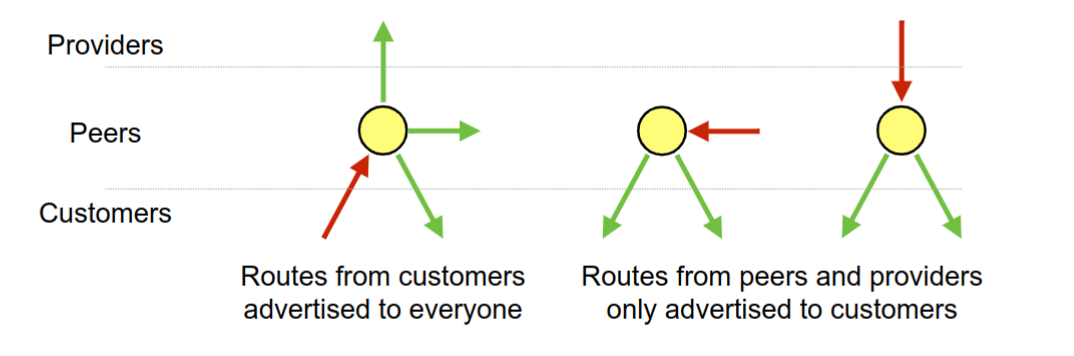
\includegraphics[width=0.5\textwidth]{assets/gao-rexford-filtering-rules.png}
    \caption{Gao-Rexford filtering rules}\label{fig:gao-rexford}
\end{figure}

Each AS exchanges routing information with neighbours.
Each AS applies policy to choose what routes to use.
Each AS applies polocy to determine what routes to advertise.

\vspace{\baselineskip}
% 9c
\textbf{Routing Security}
Any AS participating in BGP routing can announce any address prefix {-} whether or not they own it
Could accidental, or malicious.
So traffic is misdirected, this is \textbf{BGP Hijacking}.
\textbf{Resource public key infrastructure (RPKI)} is an attempt to secure internet routing.
Lets an AS make a signed \textbf{Route Origin Authorisation (ROA)} {-} a digital signature

\vspace{\baselineskip}

% 9d
\textbf{Intra-domain Routing}

Distance vector {-} the \textbf{Routing Information Protocol (RIP)}
Nodes maintain a vector containing the distance to every other node in network.
Not widely used as it is not scalable. Simple to implement, suffers from slow convergence.

Link state {-} \textbf{Open Shortest Path First routing (OSPF)}
Nodes know the links to their neighbours, and cost of using those links.
Ensures all nodes know the entire network topology.
Each nodes uses Dijkstra's algorithm to compute the shortest path to every other node.
More complex, requires each router to store complete network map. Much faster convergence.

Challenges. Construction work is good at breaking cables. Good network desings have multiple paths from source to destination.
Must quickly notice failure and switch to backup path.
\textbf{Fast failover} {-} pre-calculate alternative paths to allow rapid switchover
\textbf{Equal cost multipath routing} {-} if two paths with the same cost, alternate traffic between them
Care needed if order is important.

\clearpage

\subsection*{Past Exam Questions}

\textbf{TCP with data}
\begin{itemize}
    \item byte offset messed up
    \item ossification, syn packets dont expect data
    \item security, spoofing attacks, attacker sends malicious data in syn with forged IP address
    \item if you send data with syn and it gets lost, it complicates retransmission logic
    \item save on RTT, send instantly
\end{itemize}


\textbf{Saving congestion window}
\begin{itemize}
    \item for most cases, this will be bad
    \item connection may timeout, and go back to slow start
    \item if the new congestion window is the same size, thats perfect
    \item if the new congestion window is smaller, there will be lots of packets loss, congestion avoidance will cut the window size bu a lot
    \item if the new congestion window is larger, its okay, congestion avoidance will increase the window size (maybe slowly)
\end{itemize}


\textbf{Server push}
\begin{itemize}
    \item example is user requests html file, then server pushes the css and js files
    \item this will reduce latency as the client wont have to request the other files separately
    \item this will reduce the number of RTT times
    \item not great impact as you only save on one request to the server
    \item you could measure improvements by total time to request an html file in this example
    \item could be sending more data than the client needs
    \item this will use up bandwidth for possibly unused data
    \item if the user has cached data, then the server push will be wasted
\end{itemize}


\textbf{IPv4 vs IPv6}
\begin{itemize}
    \item future proofing
    \item more addresses, probably unnecessary
    \item routing tables will be a lot bigger when storing IPv6 addresses
    \item Open Shortest Path First routing will make it so routing tables takes up more physical memory
    \item larger headers in general
\end{itemize}


\textbf{DNS lookup}
\begin{itemize}
    \item if the client or someone near the client has requested the domain recently, then the value will be cached
    \item when the client first requests the domain, the local DNS server will make a recursive query via the DNS root server
    \item the response will also include a time to live value, which is the time period for which the value is cached
\end{itemize}


\textbf{DNS transport protocols}
\begin{itemize}
    \item DNS over HTTPS allows for making DNS queries to any server
    \item very hard to block DNS over HTTPS
    \item DNS over UDP, TCP reliability isn't needed {-} if no answer, retransmit the request, no connection
    \item DNS over TLS, slower but more secure, two handshakes
    \item DNS over TCP, slow but more secure, one handshake
    \item DNS over TCP, TLS, UDP all used a fixed resolver determined by the OS
\end{itemize}


\textbf{Multimedia data bursty behaviour}
\begin{itemize}
    \item media has a minimum rate, below which it cannot be used
    \item if the congestion control algorithm cannot sustain this rate, real-time traffic cannot be used
    \item media also has a maximum rate, cannot consume more than this, limited by frame rate and resolution
    \item frames of media data are encoded and sent periodically.
\end{itemize}

\clearpage

\textbf{Video Conference while downloading a file}

\textit{Assume the TCP connection uses the Cubic congestion control algorithm, and the network capacity is enough to comfortably transmit the video data alone without packet loss.}
\begin{itemize}
    \item during slow start, the video quality should remain high
    \item as slow start gets closer to the maximum rate, the quality will decrease,
    \item when the TCP connection gets its first packet loss, assuming a faultless connection, this will occur when the buffer of the client is full. The video quality will be at its worst.
    \item Then TCP Cubic will decrease its sending rate to 0.7 of the previous rate, so the video
    quality will increase slightly
    \item the video quality will then oscillate, getting better when the TCP connection encounters packet loss, and getting worse when the TCP connection is increasing its sending rate
\end{itemize}


\textbf{Interactive video conferencing using UDP over TCP}
\begin{itemize}
    \item UDP is lower latency, where TCP has to wait for acknowledgements
    \item UDP doesn't have build in congestion control
    \item UDP is very loss tolerant, and doesnt retransmit lost packets, useful for video conferencing as if a packets is lost, its no use later on.
    \item UDP doesnt enfore in-order delivery, so it discards out of order packets
    \item TCP with cubic could be more useful in a video call like a live lecture, where only one person is talking and streaming for most of the call, this means everyone else can recieve a reliable stream of the lecture
\end{itemize}

\textbf{Difference between intra-domain routing and inter-domain routing}
\begin{itemize}
    \item inter-domain routing is used to find the best path between two different ASes
    \item inter-domain routing is used between organisations
    \item intra-domain routing is used to find the best path within a single AS
    \item intra-domain routing is used inside an organisations network.
\end{itemize}

\textbf{Gao-Rexford filtering rules}
\begin{itemize}
    \item routes from customers advertised to everyone
    \item routes from peers and providers only advertised to customers
    \item designed to optimise profit, not routing efficiency {-} don't advertise expensive routes
    \item these restrictions help mitigate routing hijacking and prevent policy violations
    \item prevent persistant routing oscillations % chat said this?
\end{itemize}

\textbf{Explain prefix hijacking}

\textit{How can the Resource Public Key Infrastructure (RPKI) help prevent such attacks?}
\begin{itemize}
    \item prefix hijacking is when a malicious actor takes over a legitimate prefix
    \item this propagates through the global BGP routing system, leading other networks to redirect traffic to the attacker's network
    \item this can be mitigated by using RPKI to sign routes
    \item RPKI is a resource public key infrastructure, it is a way to secure internet routing
    \item also, using Route Origin Authorisation (ROA) to sign routes, this allows ASes to verify the legitimacy of routes
\end{itemize}

\textbf{Privacy concerns with using the host's link layer address as the local identifier part of an IPv6 address}
\begin{itemize}
    \item link layer addresses are globally unique and persistent, allowing tracking across different networks
    \item this makes it easier to correlate a user's activity across different networks and locations
    \item this can be used to build detailed profiles of user behavior and movement patterns
    \item this reduces anonymity as the same device can be identified regardless of network changes
    \item randomly generated link layer addresses can be used to improve privacy
\end{itemize}


\textbf{Explain why clients try to establish connections in parallel}
\begin{itemize}
    \item this will allow you to make a connection quicker
    \item this can also allow you to discover connections with faster RTTs
    \item the client may use the order of addresses returned by DNS
    \item use a staggered approach, try to connect to the first address, if not connected within 100ms, try the next one
    \item the client may also want to try a mix of IPv6 and IPv4 addresses
\end{itemize}

\textbf{How does the addition of QUIC to the network affect connection establishment}
\begin{itemize}
    \item QUIC only requires a single handshake, to establish an encrpyted connection, whereas TCP + TLS requires two handshakes
    \item QUIC is built on top of UDP, so it avoid kernel-level constraints, and QUIC provides more flexible congestion control algorithms
    \item QUIC eliminates head-of-line blocking, QUIC supports multiplexed streams, where each stream is delivered independently, so packet loss in one stream doesnt block others
    \item
\end{itemize}

\textbf{Discuss wether end-to-end recover is the right choice}
\begin{itemize}
    \item it keeps the network simple, logic is pushed to the edges
    \item easier to scale, as links do not need complex retransmission logic
    \item end hosts can optimise transport protocols independent of the network
    \item putting logic like this in the network could lead to protocol ossification, poorly implemented retransmission logic could prevent future changes
    \item end hosts have knowledge of the transmission session and can optimize retransmisson strategies accordingly
    \item reduces hardware and software costs in the network
    \item in network software could find it hard to detect packet loss on damaged physical links, leading to flakey and unpredictable behaviour, which could mean end hosts may still have to retransmit some packets
    \item although, this leads to possibly more latency, in network retransmission softwares could detect packet loss quicker and retransmit quicker than end hosts
    \item lost packets must traverse the whole link again, taking up bandwidth
\end{itemize}

\textbf{TCP Acknowledgements}

\textit{And selective acknowledgements}
\begin{itemize}
    \item A TCP acknowledgement (ACK) is sent when a packet arrives that contains new data; the
    acknowledgement number indicates next contiguous sequence number expected
    \item TCP selective acknowledgements (SACK blocks) are a TCP extension that allows a receiver
    to signal receipt of non-contiguous packets in addition to the standard ACK
    \item SACK blocks are useful because they give the sender information that it needs to avoid
    unnecessary retransmissions when a triple duplicate ACK is received
    \item SACK blocks don't affect the congestion control algorithm, they just change what packets
    are retransmitted
\end{itemize}

\textbf{TCP receive window}

\textit{impact of window scaling}
\begin{itemize}
    \item The receive window denotes the amount of buffer space the receiver has available to hold
    data received on a TCP connection
    \item The range available in the TCP header proved to be too small for receivers on high-speed
    networks so a window scale of n increases the signalled window by a factor or 2n
    to allow for larger windows
\end{itemize}


\textbf{Difference between receive window and congestion window}
\begin{itemize}
    \item The receive window is the available buffer space at the receiver
    \item the congestion window is an estimate of the available network capacity
    \item performance is limited by whichever is smaller; the receiver needs enough buffering to match the network if the
    full performance is to be reached
\end{itemize}

\textbf{Most packets in the internet are similar sizes}
\textit{large number 40 bytes, large number 1500 bytes}
\begin{itemize}
    \item packets of 40 bytes will most likely be TCP ACK packets, 20 bytes for the TCP header, 20 bytes for the IP header
    \item the maximum transmission unit (MTU) is 1500 bytes, so any packet larger than this will be fragmented
    \item most traffic patterns involve control packets or data packets, so this makes sense that few packets are not of those sizes
\end{itemize}

\textbf{Explain 0-RTT in TLS}

\textit{why it improves performance? Risks? do benefits outweigh risks?}
\begin{itemize}
    \item 0-RTT connection re-establishment works by sharing a key in one session
    (the PreSharedKey), that is then used to send encrypted data along with the initial
    TLS ClientHello message in the following session
    \item 0-RTT connection re-establishment improves performance because it allows an ini-
    tial request to be sent to the server along with the first TLS handshake packet (the
    ClientHello), and for the reply to be included with the ServerHello, removing one RTT
    \item The risks with 0-RTT re-establishment is that any data sent along with the
    ClientHello is subject to reply attacks, and is not forward secret since it
    reused a key from the previous session
    \item  Whether the benefits of 0-RTT connection re-establishment outweigh the cost is a
    judgement call, and answers may legitimately argue in either way. There is
    available for stating an opinion, and for providing a reasoned justification.
\end{itemize}

\clearpage

\textbf{Why are QUIC headers encrypted?}
\begin{itemize}
    \item QUIC encrypts transport headers to protect privacy and to prevent protocol
    ossification
    \item the privacy concern is to avoid metadata leakage that exposes sensitive information about participants.
    \item governments and other organisations may want to monitor this data
    \item a TCP-related example would be that an observer who can see packets and their
    acknowledgements can infer distance from sender to receiver based on packet timing,
    and this is known to be useful for geolocation. A TLS-related example would be that
    the Server Name Indication (SNI) field is unencrypted.
    \item  The key point around ossification is that devices in the network soon start of rely on the
    presence, and format, of exposed transport header fields. This makes it diffi-
    cult to change the protocol after initial deployments. Any reasonable example
    of ossification is accepted, including difficulties extending TLS version negotiation for
    TLS 1.3 or the introduction of SACK blocks or ECN\@.
\end{itemize}

\textbf{Why is the threshhold for retransmission of lost packets in TCP set to 3?}
\begin{itemize}
    \item Delayed packets cause duplicate sequence numbers. The threshold
    is chosen to be three duplicate acknowledgements because otherwise packet reordering
    would cause unnecessary retransmission.
    \item The threshold of three consecutive duplicate acknowledgements was chosen based on
    measurements of the packet loss and reordering in the network. Reordering
    of consecutive packets is common enough to be worthwhile accommodating in the
    protocol; further reordering is not.
    \item Setting the threshold to two duplicate acknowledgements would make it more likely
    that the sender would retransmit a packet unnecessarily in response to packet reordering
    \item Setting the threshold to four duplicate acknowledgements would make it more likely that
    a retransmission would be unnecessarily delayed when a loss has occurred.
\end{itemize}


\textbf{Explain explicit congestion notification (ECN)}
\begin{itemize}
    \item ECN is a signal that the network is starting to become congested, but is not
    yet sufficiently overloaded that packets need to be discarded.
    \item The sender sets the ECN bits in the IP header to ECT (0) or ECT (1) to indicate that it
    supports ECN\@.
    \item If there is congestion, some router within the network changes
    will change this to ECN-CE to inform the receiver.
    \item On receipt of an ECN-CE mark, a TCP receiver sets the ECN Echo (ECE) bit in the
    TCP header of the segment it generates to acknowledge that data.
    \item On receipt of a TCP segment with the ECE bit set, the sender reduces its congestion
    window in the same way it would if a packet was lost.
\end{itemize}


\textbf{Why is ECN beneficial for interactive conferencing?}
\begin{itemize}
    \item ECN feedback allows the sender to react to congestion early, so UDP packet
    loss can be avoided. This improves quality of the audio and video, since UDP
    is unreliable and doesn't retransmit lost packets.
    \item In addition, since the router queues are no longer full to overflowing, the queueing
    latency within the network is reduced. This is beneficial for interactive video
    conferencing, since latency makes an interactive call difficult.
\end{itemize}

\textbf{What would happen if the DNS root servers failed?}
\begin{itemize}
    \item The important point here is that DNS records have a TTL and are widely
    cached. Accordingly, things would keep working as before the failure until
    the cache entries time out, although applications would immediately be unable
    to lookup new names that were not in the cache. You'd therefore expect to
    see a gradual increase in DNS lookup failures over time, as the cache entries expire.
\end{itemize}

\textbf{Why was DNS deployed over UDP a good idea?}

\textit{why they are changing?}
\begin{itemize}
    \item UDP used to be a good choice because it was fast and low overhead since the
    request and response would each fit into a single packet.
    \item TCP offers no benefit in terms of reliability compared to just resending a request if no answer is received, and there is not enough data for congestion control to work.
    \item DNS is moving to alternative transport protocols because: (1) With the deployment
    of DNS security and authenticated DNS responses, DNS replies are now too large to
    fit into a single UDP packet [2 marks]; (2) It is desirable to encrypt and authenticate
    \item DNS requests and responses, and this is easier to do is running over some transport that
    provides these features (e.g., TLS over TCP).
\end{itemize}

\textbf{Explain what is DNS-over-HTTPS and why its controversial}

\begin{itemize}
    \item DNS-over-HTTPS is DNS requests sent within HTTPS to some server within
    the network that can perform the DNS lookup and send the reply within the HTTPS
    response.
    \item It's controversial because it circumvents the local DNS resolver and any policy that
    resolver with enforce, and because there are privacy implications with a
    central DNS resolver that can track queries.
    \item Up to are available for broader discussion of these issues and whether
    deployment of DNS-over-HTTPS is a good idea. Answers may legitimately argue for
    or against this proposition. Likely answers are that DNS-over-HTTPS is beneficial
    because it protects against phishing attacks from malicious local resolvers; equally, it
    might be harmful because it prevents local resolvers from applying desirable policies or
    local laws that the central server is unaware of. Marks will be assigned for reasoned
    technical argument.
\end{itemize}

\textbf{Locating the nearest CDN using DNS vs anycast}

\textit{When large number of people and geographical locations are changing rapidly}
\begin{itemize}
    \item Both must use the resolver to get the IP address of the CDN
    \item DNS will have a lot of load
    \item DNS routing uses the DNS to locate the nearest CDN
    \item local caching will mean some users will locate a CDN not close to them
    \item anycast will always locate the nearest CDN, using BGP
\end{itemize}


\end{document}
